\chapter{绪论}

\section{研究背景和意义}
近几年,知识图谱(Knowledge Graph)作为一种结构化的知识存储形式被众多信息检索系统作为不可或缺的基础组件而广泛使用 \cite{zou2020survey}。语义网络的概念最早可追溯到2001年Berners-Lee的相关研究 \cite{berners2001semantic},他主张推动和发展知识表示相关的如资源描述框架(RDF)等技术的标准。早期类似基于图的知识结构广泛采用RDF标准进行表示,而随着互联网的出现及发展,语义网络开始转向语义互联网发展,并在2012年由谷歌提出名为知识图谱的新兴技术并应用在搜索引擎上。

知识图谱是使用图结构来描述知识的知识库。知识图谱由节点和边组成,其组成可以涵盖实体、概念、关系、属性等,作为一种结构化知识表示的形式,他将现实中的知识通过节点及节点间关系组成图来进行结构化的表示。一方面,知识图谱以图的形式将抽象的知识形象化的表示更直观地展示出知识的相互联系和内容,同时利用高效的图遍历算法可以完成对知识更全面的检索和查询;另一方面,知识图谱可以从数据中识别、推理、发现实体间及实体与概念间的复杂关系,将存储的知识转化为可计算的模型,凭此辅助进行知识问答、推荐系统等丰富的下游任务,如在电商系统中,通过对用户偏好图谱的构建可以更好的预测用户的购买意向进行相关商品推荐从而收获更好的经济效益。虽然知识图谱广泛使用的三元组存储已经可以将知识进行高效的结构化表示,但是这种传统的符号形式的表示仍旧会导致知识图谱在使用上备受局限。

为了解决这个问题,知识图谱表示的相关研究很快起步并获得了广泛的关注。知识图谱表示学习(Knowledge Representation Learning,也称知识图谱嵌入)旨在将符号化的三元组(h, r, t)映射到低纬稠密的向量空间,便于实体和关系之间的计算 \cite{JSYJ202103003},降维后获得的知识图谱嵌入可以作为其他网络模型的输入来辅助下游任务的效果提升,包括知识图补全(KGC)、三元组分类、实体识别、关系抽取以及图谱外任务如推荐系统、问答系统等,例如谷歌构建的规模庞大的知识图谱也已经展示出该方法的强大能力。但当下表示学习的方法仍无法顾及到所有的应用场景,具有一定的使用局限性。

在传统的知识图谱表示学习应用场景下,学习的目标是获得知识图谱中的实体和关系最优的降维编码,而后可以利用这些编码进行下游的任务;其中任务中涉及的实体及关系往往是模型训练阶段都可以接触到的(称为可见实体、可见关系)。经典的KGE模型如基于翻译的TransE \cite{bordes2013translating}模型在同一空间向量中嵌入实体,通过头实体和尾实体的平移操作来进行关系嵌入,时空复杂度低,但在建模复杂关系的场景下弊端也比较明显,为此TransE相关的扩展模型 \cite{wang2014knowledge}也陆续被研究应用。其他的KGE模型如基于分解的模型DistMult \cite{yang2014embedding}、CompleEx \cite{trouillon2016complex}以及旋转模型RotatE \cite{sun2019rotate}等也都获得了广泛的关注和应用。

\begin{figure}
  \centering
  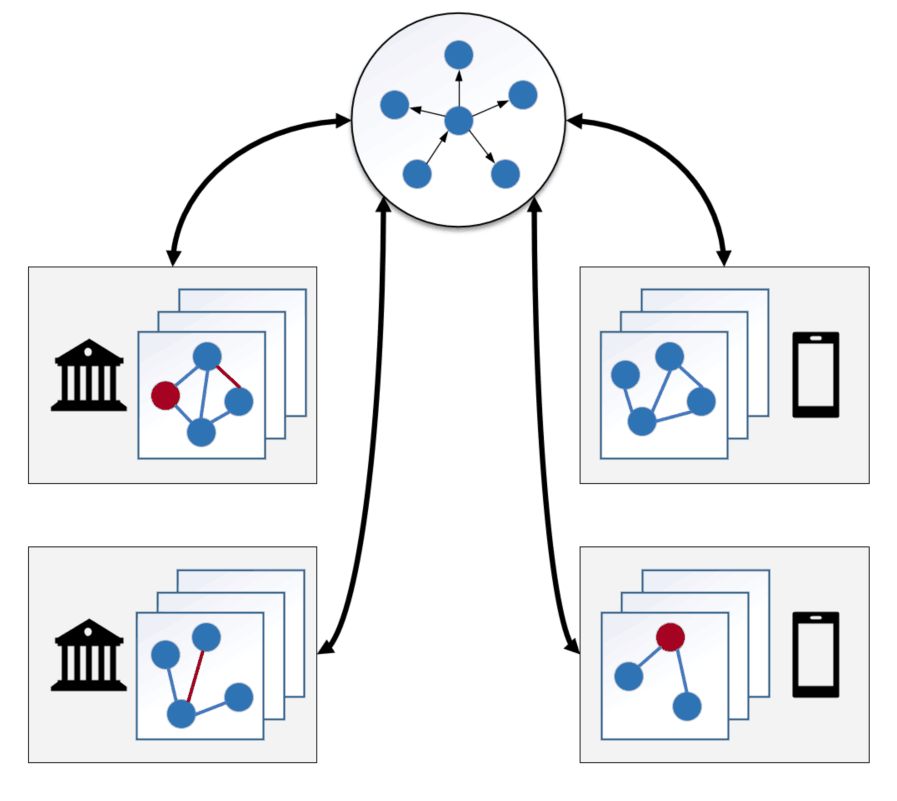
\includegraphics[width=0.6\textwidth]{1-1.png}
  \caption{跨设备下的知识图谱分布}
  \label{fig:1-1}
\end{figure}

随着知识图谱的规模越来越庞大,单机的模型训练已经满足不了更加复杂的模型需要,因此知识图谱被逐渐部署在多台设备上并行处理来提高计算的效率,同时这些分散的图谱数据因为规模、成本等原因无法进行很有效的统一知识合并,而这些分散的跨设备的知识图谱会随着用户使用不断的进行更新和扩充,新的实体和关系会使基于传统的表示学习模型的效果下降。现如今个人移动设备的性能越发强大,为每个客户提供最符合个人爱好的个性化服务也是服务提供商的竞争优势之一,这种在目标图谱中同时包含已知实体、已知关系、未见实体、未见关系,本文称之为跨设备场景下的知识图谱。如何在跨设备的场景下的知识图谱上设计出一套高效的图谱嵌入模型,使得该模型能够尽可能满足新兴知识图谱的需要就成为了未来发展及现实需要的很重要的待解决命题。

为了处理知识表示遇到的未见关系和未见实体的问题,相关的归纳知识图谱表示方法研究也取得了一定的效果。Ren \cite{li2022does}团队通过对语义证据的预测及实验验证研究了KGE的外推问题,通过建模对三种语义证据的加强,在知识图谱补全任务上预测不可见数据时都取得了更好的表现效果。此外Teru \cite{teru2020inductive}等人通过切分实体子图分析子图的关系信息来获得实体表示,可以对包含未见实体的关系进行预测,但目前仅针对包含未见实体的任务,可以同时处理未见实体和未见关系的知识图谱表示模型缺少且效果不佳。因此本文提出了一种融合知识图谱结构信息和本体语义信息的知识图谱表示学习模型,可以同时对数据中的未见关系和未见实体进行表示学习并取得不错的效果。

\section{国内外研究现状及趋势}
知识图谱表示学习一般包含三个步骤:1、初始化实体和关系的低纬表示,其中实体通常表示为目标空间中的向量点,关系通常表示为空间中的操作如向量、张量、矩阵等。2、定义一个统一的得分函数,将图谱中的实体和关系组合形成多个三元组,对任意一个三元组可根据该得分函数计算出得分,一般来说在知识图谱中已知的事实三元组的得分应该最高。3、学习实体和关系的表示,通常采用梯度下降的方式求解。其中根据评判标准的不同,得分函数大体上分为三类:基于翻译的方法、基于语义相似度的方法以及融合辅助信息及归纳推理的方法。本节将分为三小节简单介绍相关的研究现状及趋势。

\subsection{基于翻译的方法}
知识图谱表示学习的关键是学习出实体和关系特征的低纬度表示,这些表示空间主要是指逐点空间,具体的像向量、矩阵和张量等表现形式;而其他类型的表示空间,如复向量空间、高斯空间也被研究者所使用 \cite{dai2020survey}。基于翻译的方法通过测量实体向量间的距离来计算出三元组事实的可信度。这些基于翻译的方法通常会将关系的嵌入视为从头结点到尾结点的向量平移,例如Bordes等研究者在借鉴Word2Vec \cite{mikolov2013distributed}中的语义平移后提出的TransE模型认为在同一表示空间中头结点向量和关系向量的向量和在距离上应该更靠近事实上的尾结点,并以此设置评分函数进行图谱嵌入,在WordNet和FreeBase两个数据集上的链接预测任务的效果相比于早期的RESCAL \cite{nickel2011three}模型会更好。同时由于TransE模型结构并不复杂,实现简单,在学术界和工业界都获得了广泛的研究及使用,使其成为经典的知识表示学习方法之一。
\begin{figure}[h]
  \centering
  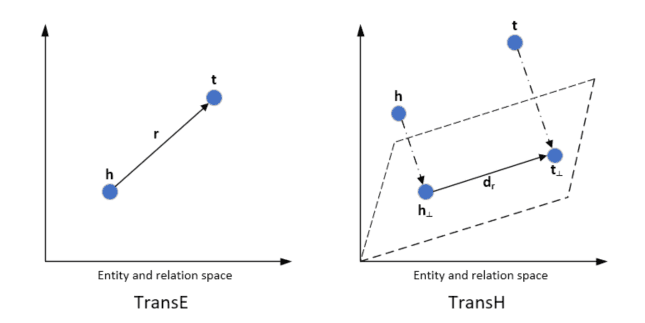
\includegraphics[width=0.8\textwidth]{1-2.png}
  \caption{TransE和TransH的实体关系映射}
  \label{fig:1-2}
\end{figure}

Bordes提出了关系的四种类型:1对1、1对多、多对1、多对多。TransE通过比较头结点与关系的向量和与尾结点的距离能够有效的处理1对1的简单关系类别,但同时缺点也显而易见,在处理复杂关系时由于实体或者关系嵌入的相似性会导致实验效果的下降。假设建模1对多的复杂关系,有(海贼王,人物,梦奇·D·路飞),(海贼王,人物,娜美)两个三元组,在同一个表示空间中,由于实体h和关系r相同,TransE会认为对应的所有尾实体都应该具有极为相似的向量表示,但很明显这个结论与事实相悖。为了弥补TransE模型的弊端,在该模型的基础上,相关的模型研究也有更新的发展。TransH通过将头尾实体都映射到关系的超平面上,即使头实体和关系一致也不会导致尾实体的嵌入一致,规避了尾结点重叠的问题,可以在一定程度上处理多对多的关系。
\begin{figure}[h]
  \centering
  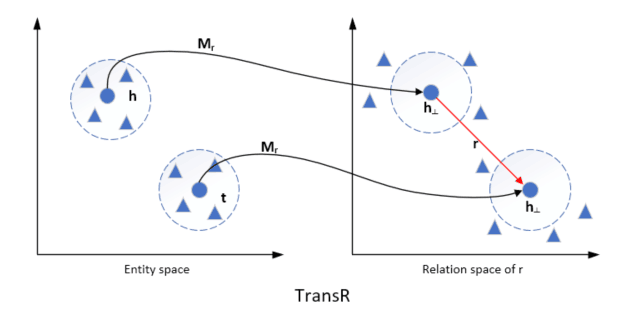
\includegraphics[width=0.8\textwidth]{1-3.png}
  \caption{TransR的实体关系映射}
  \label{fig:1-3}
\end{figure}
\begin{figure}[h]
  \centering
  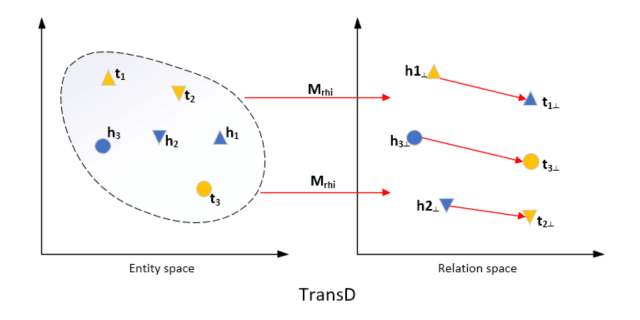
\includegraphics[width=0.8\textwidth]{1-4.png}
  \caption{TransD的实体关系映射}
  \label{fig:1-4}
\end{figure}

TransR \cite{lin2015learning}舍弃了实体和关系映射在统统一语义空间中的假设,把TransH涉及到的实体在关系上特有的映射的概念延展成关系特有的语义空间映射,在TransR的设定中三元组的实体映射到一个语义空间,而关系则表示为关系语义空间中的转换向量,TransR定义了关系关联的映射矩阵, 在执行转移操作之前, 分别通过实体向量在关系映射矩阵上的映射获得关系空间内的头实体与尾实体表示, 最后通过计算头实体映射向量加关系向量和尾实体映射向量的距离得到优化目标。但TransR模型将实体语义空间与关系语义空间的交互仅仅与关系矩阵相关联明显不合理,且由于空间投影使模型参数急剧增加,基于此Ji等人提出了TransD \cite{ji2015knowledge}模型,TransD模型设置了两个投影矩阵,分别将头实体和尾实体投影到关系空间,同时只利用两个投影向量构建投影矩阵来减少参数量。

总体上,基于翻译的Trans模型都将关系作为实体向量间的翻译,但受限于结构的弊端往往不能很好处理复杂关系的场景,无法得到蕴含更多特征的知识图谱表示。

\subsection{基于语义相似度的方法}
基于语义相似度的方法通过标记实体和关系在向量空间表示所隐藏的语义特征的相似程度来作为评判三元组合理性的标准。传统的的语义匹配的模型一般采用张量分解的方式来完成,其中的张量由一个多维的数组来表示 \cite{kolda2009tensor}。
\begin{figure}[h]
  \centering
  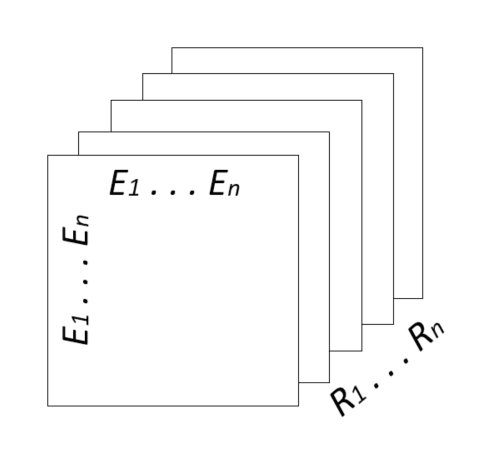
\includegraphics[width=0.5\textwidth]{1-5.png}
  \caption{知识图谱的张量模型}
  \label{fig:1-5}
\end{figure}

RESCAL模型将每个实体与一个向量联系起来,以捕捉其潜在的语义。每一种关系都用一个矩阵来表示,该矩阵模拟了潜在因素之间的双向相互作用。该模型通过潜在特征的成对交互解释三元组,首先将知识图谱中的三元组转换为三维张量\(X\)。给定一个张量\(X \in R^{n×n×m}\),其中\(n\)和\(m\)分别表示实体和关系的数量,该张量的两个模保存连接的头尾实体,另一个模则保存关系。如果一个张量实体\(X_{ijk} = 1\)即表明知识图谱中存在三元组(第i个实体,第k个关系,第j个实体);否则,\(X_{ijk} = 0 \)表示不存在或未见的三元组。然后对张量的每一个切片(关系数据)执行分解来获得实体的潜在语义表示,然而该模型的主要缺点在于对频繁出现的关系表现的很好,但对少见的关系表现的很差,并且容易导致过拟合,不适用存在大量稀有关系的数据集 \cite{choudhary2021survey}。鉴于此,研究者提出了一个潜在因子模型TATCE \cite{garcia2014effective},它能够将高容量三向模型与更易于控制的双向交互模型相结合,并利用它们两者的优势。由于双向和三向模型不使用相同的数据模式,也不在嵌入中编码相同的信息,因此在TATEC中,他们在第一阶段使用了两种不同的嵌入,然后在后期将它们组合并微调。相比于三向模型RESCAL、传统双向模型TransE以及同样采取双向三向模型结合的NTN \cite{socher2013reasoning}模型等,在链接预测任务上TATEC表现更优。为了简化模型计算的复杂度,DistMult模型在RESCAL的基础上将关系矩阵简化为对角矩阵,从而减少双线性模型的参数量,达到和TransE基本相同。ComplEx模型是对DistMult在关系模式上的改进,不仅具有学习对称关系的能力,还能够提供一些非对称性的表示。

近几年随着神经网络的兴起,由于其具有强大表示和泛化能力,也可以表达复杂的非线性投影。结合神经网络将知识图嵌入到连续的特征空间成为一个热门方向。其中代表性的如ConvE\cite{dettmers2018convolutional}、ConvKB\cite{nguyen2017novel}模型等,这些早期的结合神经网络模型的KGE方法采用卷积神经网络进行特性提取及嵌入,通过卷积神经网络捕捉知识库中的全局关系和翻译特性。将三元组输入到卷积层中进行卷积操作,输出特征并拼接为特征向量,然后经由评分函数进行打分。随着图卷积模型\cite{kipf2016semi}的提出及效果的不断提升,以图卷积网络为基础的KGE模型开始占据主流。R-GCN\cite{schlichtkrull2018modeling}首次提出采用图卷积网络做图谱嵌入任务,使用GCN的信息传播的思想表示图谱,并用上层的卷积输出作为下层的卷积输入。虽然R-GCN 的效果提升都比较微弱,但是因为GCN的出现,用它来做知识图谱表示学习也成为是一种必然。此后,基于GCN的KGE模型如CompGCN\cite{vashishth2019composition}也已经取代传统的神经网络KGE模型,不断取得更好的知识图谱嵌入效果。

\subsection{融合辅助信息及归纳推理的方法}
基于翻译的表示学习方法和基于语义相似度的表示学习方法通过三元组信息学习实体及关系的表示。这些方法的目的都是学习知识图谱存储的事实信息并映射到嵌入向量中,使嵌入向量能够更好地贴近这些事实,从而完成各种下游任务。然而,这些仅依赖于知识图谱三元组进行表示学习的方法存在明显的弊端。这些学到的嵌入表示只能处理知识图谱中可见的实体和关系,对于未见组件可靠性会大幅下降。为了能够对这些未见的组件进行有效的特征学习,研究者往往会引入除三元组之外的辅助信息。因为知识图谱不仅通过三元组进行数据存储和检索,还蕴含着丰富的其他信息可以辅助进行知识图谱表示学习,比如文本描述信息、关系路径信息及图结构信息等。

NTN模型最早在表示学习中引入实体的描述信息。虽然该模型是利用图谱存储的实体的文本信息来对实体嵌入进行初始化操作。此后描述扩展的知识图谱表示模型DKRL \cite{xie2016representation}试图通过改进TransE模型使其能够进一步处理实体描述,DKRL将实体嵌入由实体结构相关的变量及实体描述相关的变量联合表示,其中实体描述变量由描述文本通过连续词袋 \cite{valverde2012link}编码器或卷积神经网络编码器获得的词嵌入构成。另一种常见的辅助信息通过借助实体的关系信息来进行表示学习,关系信息揭示了实体之间的一个或多个语义关系。PtransE \cite{lin2015modeling}首次将图谱的多跳关系信息作为知识图谱嵌入的辅助信息,提出了一个以关系路径为基础的表示学习模型。该模型在TransE基础上改进,模型打分函数由两个部分组成,一方面是头尾实体直接关系的打分,另一方面计算头尾实体间其他多跳关系路径的打分。从而将transE的单步推理扩展为多步,获得了不错的效果提升。冯俊等人则将知识图谱视为一个大的有向图,提出了基于图感知的表示模型GAKE \cite{feng2016gake}。该模型利用知识图的结构信息生成实体和关系的表示。
\begin{figure}[h]
  \centering
  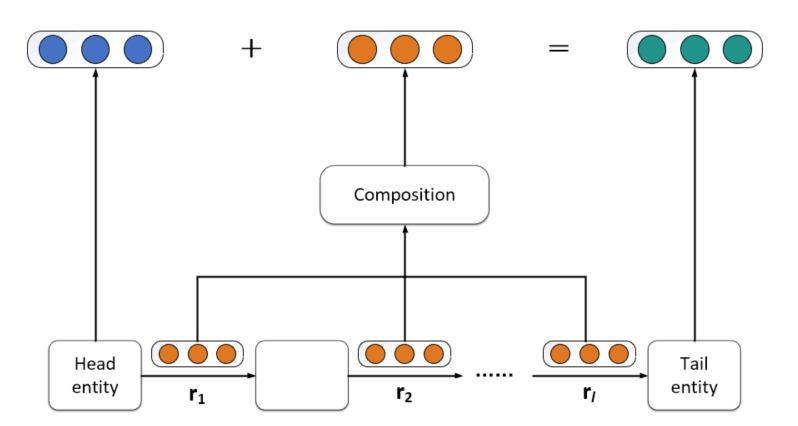
\includegraphics[width=0.7\textwidth]{1-6.png}
  \caption{PtransE的模型架构}
  \label{fig:1-6}
\end{figure}

除了知识图谱自身的额外信息作为辅助外,许多研究者也会引入图谱外的其他知识用于表示学习。比如上述的实体描述信息,也可以从新闻稿或者维基百科中获取。图谱外其他模态的信息也同样被用于辅助表示学习,比如实体的图像信息,代表性的IKRL \cite{xie2016image}模型实现了包含基于跨模态结构和基于图像的表示,将图像编码到实体空间同时遵循平移原则。该模型提出的跨模态表示可以确保基于结构的表示和基于图像的表示映射在在同一个表示空间中。

以往的知识图谱表示学习聚焦于如何从现有的图谱知识中学习到更贴近知识的嵌入表示来完成相关的预测、补全、问答等任务,但这些学习往往学习到的不是更全局的表示,仅在现有的可见的图谱任务上才能获得较好的效果。而跨领域跨设备的场景要求更加苛刻的表示学习效果,需要更高层次、更适用性的知识提取,因此现有的研究开始向通用性知识以及辅助知识提取方向发展,该方向研究正在起步但无疑是未来的主要方向,本文的研究目标即在高层本体语义信息的辅助下进行更普适性的知识图谱表示学习。

\section{本文主要研究内容}
针对跨设备场景下知识图谱表示学习的调研不难发现传统的知识图谱表示学习方法无法很好处理未见的组件,而通过融合其他辅助信息来对未见组件表示的方法往往只能聚焦于某一类未见组件,而不能处理同时存在未见实体和未见关系的情况;同时在跨设备的场景要求下大大加强了对模型泛化性的要求,因此本文总结出以下两个主要面临的难题:

\begin{enumerate}[label=\arabic*)]
  \item 传统的知识图谱嵌入方法无法有效处理未知的实体和关系。当采用使用归纳推理的模型时,往往需要依赖规则和结构信息来处理单一未知组件,这些方法通常在子图的结构信息中学习未知组件的表示,但忽略了知识图谱中丰富的语义信息。如何在归纳推理模型中嵌入有效的语义信息是当前研究的一个难点。

  \item 对于跨设备下的知识图谱表示学习,模型需要在训练数据集上训练获得参数,以使其在存在未见组件的新型知识图谱上也可以正确地发挥作用。然而,在采用分散知识图谱存储方式时,需要思考如何进行模型训练,并在其训练中设置未见组件以帮助模型获取更强大的泛化性能,以更好地满足现实场景下的需求。
\end{enumerate}

% 本文通过对近几年相关技术的研究认为,本体作为知识图谱最高层次的语义抽象可以作为所有设备的全局信息,可以用于对未见关系和未见实体进行一定程度上语义特征的补充。同时借助于关系的位置关系,通过实体三元组关系与关系的相对关系构建出关系位置图,然后在该图中嵌入本体的语义信息,能够对关系节点进行编码从而学习到未见关系的特征表示;然后基于实体及连接关系的结构信息,可以通过未见实体连接的所有关系,聚合这些关系的特征作为实体特征从而实现了对未见实体的表示;最后,为了模拟出存在未见关系及未见实体的训练场景,本文借用元学习的思想设计了多个训练任务学习到最好的模型参数并进行实验验证了模型的有效性。

本文通过对近几年相关技术的研究认为,本体作为知识图谱最高层次的语义抽象可以作为所有设备的全局信息,并可用于对未知关系和实体进行一定程度的语义特征补充。此外,通过确定关系的相对位置关系,可以构建关系位置图,并嵌入本体的语义信息,从而对关系节点进行编码,以学习未见关系的特征表示。而后,基于实体及连接关系的结构信息,可以聚合连接未知实体的所有关系的特征,以表示未知实体。最后,为了模拟出具有未知关系和实体的训练场景,本文借用元学习的思想设计了多个训练任务,以学习最佳模型参数,并通过实验验证了模型的有效性。

综上,本文的研究内容主要有以下几个方面的贡献:
\begin{enumerate}[label=\arabic*)]
  \item 分析了跨设备知识图谱表示学习当下遇到的一些问题及相关研究方法的一些进展,提出了一个融合了本体语义信息同时对未见关系和未见实体进行表示学习的嵌入学习模型框架。

  \item 引入元学习的模型训练方法,设置多个单任务的训练任务,在各个任务中引入未见关系和未见实体用于模型训练,使得模型能够在单个训练集上训练并且能够快速作用在测试图谱上,获得更强的模型泛华能力。

  \item 在多个数据集上进行了丰富的模型测试并与其他基准模型结果进行对比分析,验证了模型的有效性;同时通过一系列消融实验验证模型各部分的重要性,为之后的模型改进提供思路和支撑。
\end{enumerate}

\section{本文组织结构}
本文的内容分为五章,以下主要概括各章的内容及安排:

第一章,绪论部分:主要介绍跨设备下的知识图谱表示学习相关的研究背景和现实意义,结合国内外研究者的相关研究分别介绍了传统的知识图谱表示学习方法中的基于翻译和基于语义相似度的方法以及相关一些通过辅助信息和归纳推理解决未见组件的一些研究进展,最后总结了研究面临的问题及本文的解决思路。

第二章,相关技术研究:分三个小结介绍了本文模型主要涉及到的三种技术的发展状况及原理分析。其中本体信息作为本文模型主要的语义信息来对未见组件进行语义层次的补充;元学习训练方法已经被广泛运用在各个领域,本文介绍了涉及到的设计方法;最后本文模型作为归纳推理模型的延伸,介绍了归纳推理模型相关的研究进展。

第三章,基于元学习本体增强的跨领域知识图谱表示模型介绍:详细介绍了本文提出的知识图谱归纳表示学习模型的各个组成部分,主要包含了本体信息嵌入模块、关系结构图构建及基于GCN的关系特征学习、基于CompGCN的实体特征学习模块。学习到实体和关系的相关表示后采用多种KGE得分函数来进行打分和更新。最后说明了模型在进行元学习训练的任务设定及训练流程。

第四章,实验结果及分析:介绍了本文采用的可用于归纳推理知识表示学习任务评测的三个数据集的构建方法以及相关用于本体嵌入的本体三元组抽取的方法。本章将本文模型及相关基准模型在目标数据集上进行了充分的实验并比较实验结果,验证了模型的有效性。最后对本文模型的各组成模块进行消融实验,验证了各模块的重要性。

第五章,总结部分:综合全文的研究内容及实验结果,总结了模型的可取部分及仍存在的问题与可改进的方法,对未来的相关工作进行规划。